\textbf{Постановка задачи.}
Исследование из области солнечной энергетики\cite{litlink1}. На Рис. \ref{ris:image1} показана схема установки для исследования фотоэлектрических характеристик.

\begin{figure}[H]
	\center{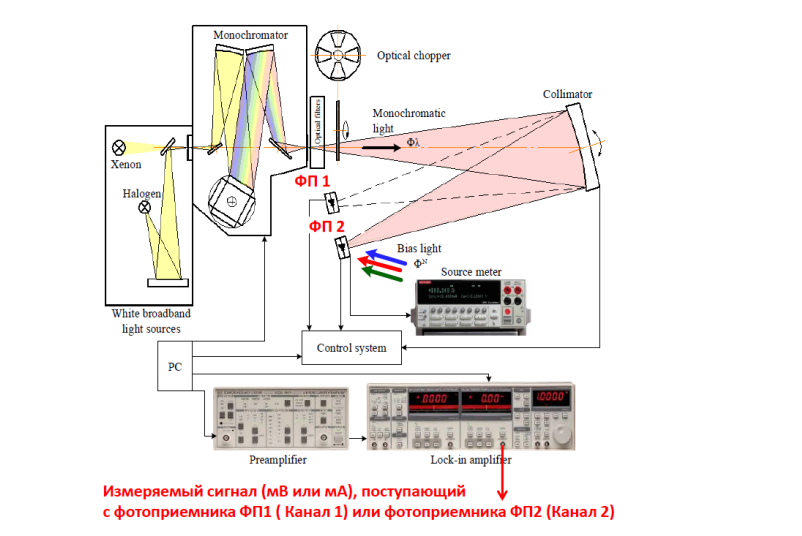
\includegraphics[width=0.5\linewidth]{images/scheme.png}}
	\caption{Схема установки для исследования фотоэлектрических характеристик.}
	\label{ris:image1}
\end{figure}

Калибровка датчика ФП1 производится по этилону ФП2. Зависимость между квантовыми эффективностямдатчиков предполагается постоянной для каждой пары наборов измерений (\ref{eq1})

\begin{equation} \label{eq1}
    QE_{\text{ФП2}} = \frac{I_{\text{ФП2}}}{I_{\text{ФП1}}} \cdot QE_{\text{ФП1}}.
\end{equation}

$QE_{\text{ФП1,2}}$ - квантовыми эффективностями эталонного и исследуемого датчика, $I_{\text{ФП1,2}}$ - измеренные токи.

\textbf{Исходные данные.}
Имеется 2 выборки данных с интервальной неопределенностью. Одна из них относится к эталонному датчику ФП2. Другая выборка соответствует исследуемому датчику ФП1. Данные представлены в виду двух текстовых файлов с числом отсчетов 50-200.

Названия файлов имеют формат:\\
$FN1='\text{Канал } 1\_700nm_0.03.csv',$\\
$FN2='\text{Канал } 2\_700nm_0.03.csv'.$\\
Здесь 700 и 0.03 указывают на условия проведения измерений.